% This must be in the first 5 lines to tell arXiv to use pdfLaTeX, which is strongly recommended.
\pdfoutput=1
% In particular, the hyperref package requires pdfLaTeX in order to break URLs across lines.

\documentclass[11pt]{article}

% Remove the "review" option to generate the final version.
\usepackage{acl}

% Standard package includes
\usepackage{times}
\usepackage{latexsym}
\usepackage{graphicx}

% For proper rendering and hyphenation of words containing Latin characters (including in bib files)
\usepackage[T1]{fontenc}
% For Vietnamese characters
% \usepackage[T5]{fontenc}
% See https://www.latex-project.org/help/documentation/encguide.pdf for other character sets

% This assumes your files are encoded as UTF8
\usepackage[utf8]{inputenc}

% This is not strictly necessary, and may be commented out,
% but it will improve the layout of the manuscript,
% and will typically save some space.
\usepackage{microtype}

%%%%%%%%
% \usepackage{blindtext}
\usepackage{xcolor,soul}
\usepackage{tabularx}
\usepackage{longtable}
\usepackage{multirow}
\usepackage{arydshln} %for h-dotted lines in table
% \usepackage{todonotes}
% \usepackage{cite}
\usepackage{hyperref} 
\usepackage{tablefootnote}
% \pagenumbering{roman}


\newcommand{\model}{\texttt{our model}}  % not used
\newcommand{\dataset}{\texttt{ClaVer}}
% If the title and author information does not fit in the area allocated, uncomment the following
%
%\setlength\titlebox{<dim>}
%
% and set <dim> to something 5cm or larger.

\title{Document Retrieval and Claim Verification \\to Mitigate COVID-19 Misinformation}

% Author information can be set in various styles:
% For several authors from the same institution:
% \author{Author 1 \and ... \and Author n \\
%         Address line \\ ... \\ Address line}
% if the names do not fit well on one line use
%         Author 1 \\ {\bf Author 2} \\ ... \\ {\bf Author n} \\
% For authors from different institutions:
% \author{Author 1 \\ Address line \\  ... \\ Address line
%         \And  ... \And
%         Author n \\ Address line \\ ... \\ Address line}
% To start a seperate ``row'' of authors use \AND, as in
% \author{Author 1 \\ Address line \\  ... \\ Address line
%         \AND
%         Author 2 \\ Address line \\ ... \\ Address line \And
%         Author 3 \\ Address line \\ ... \\ Address line}



% \author{Megha Sundriyal \\ 
%         IIIT-Delhi, India \\ 
%         \texttt{meghas@iiitd.ac.in} \\ 
%         \And
%         Ganeshan Malhotra\\
%         BITS Pilani, Goa, India\\
%         \texttt{f20170512g@alumni.bits-pilani.ac.in} \\
%         \And 
%         Md Shad Akhtar\\
%         IIIT-Delhi, India \\
%         \texttt{f20170512g@alumni.bits-pilani.ac.in} \\}

\author{Megha Sundriyal$^1$, Ganeshan Malhotra$^2$, Md Shad Akhtar$^1$, Shubhashis              Sengupta$^3$, \\ {\large \bf Andrew Fano$^3$, Tanmoy Chakraborty$^1$}\\
        $^1$\textit {IIIT-Delhi, India}, 
        $^2$\textit{BITS Pilani, Goa, India},
        $^3$\textit{Accenture Labs, India} \\
        meghas@iiitd.ac.in,  f20170512g@alumni.bits-pilani.ac.in, shad.akhtar@iiitd.ac.in,\\
        shubhashis.sengupta@accenture.com, andrew.e.fano@accenture.com, tanmoy@iiitd.ac.in
        }

% \author{{Megha Sundriyal$^1$, Ganeshan Malhotra$^2$, Md Shad Akhtar$^1$, Shubhashis Sengupta$^3$,\\ {\large \bf Andrew Fano$^3$, Tanmoy Chakraborty$^1$}}} 


% \address{$^1$\textit {IIIT-Delhi, India}
%       $^2$\textit{BITS Pilani, Goa, India}
%       $^3$\textit{Accenture Labs, India}\\
%       meghas@iiitd.ac.in,  f20170512g@alumni.bits-pilani.ac.in, shad.akhtar@iiitd.ac.in,\\
%       shubhashis.sengupta@accenture.com, andrew.e.fano@accenture.com, tanmoy@iiitd.ac.in}



\begin{document}
\maketitle
\begin{abstract}
During the COVID-19 pandemic, the spread of misinformation on online social media has grown exponentially. Unverified bogus claims on these platforms regularly mislead people, leading them to believe in half-baked truths. The current vogue is to employ manual fact-checkers to verify claims to combat this avalanche of misinformation. However, establishing such claims' veracity is becoming increasingly challenging, partly due to the plethora of information available, which is difficult to process manually. Thus, it becomes imperative to verify claims automatically without human interventions. To cope up with this issue, we propose an automated claim verification solution encompassing two steps -- document retrieval and veracity prediction. For the retrieval module, we employ a hybrid search-based system with BM25 as a base retriever and experiment with recent state-of-the-art transformer-based models for re-ranking. Furthermore, we use a BART-based textual entailment architecture to authenticate the retrieved documents in the later step. We report experimental findings, demonstrating that our retrieval module outperforms the best baseline system by 10.32 NDCG@100 points. We escort a demonstration to assess the efficacy and impact of our suggested solution. As a byproduct of this study, we present an open-source, easily deployable, and user-friendly Python API that the community can adopt. 
\end{abstract}

\section{Introduction}
The escalating drift of online social media platforms has led to a massive rise in online content consumers. Participation in these platforms has swung into another correspondence, which is no longer limited by physical barriers. Because of their speed and focused information, these platforms facilitate the dissemination of personal thoughts and information to a much larger audience. However, at the same time, these platforms have enriched an equally docile environment for malicious users to promulgate fake news, bogus claims, rumors and misinformation. There have been numerous cases where the propagation of malicious unverified content has influenced the entire society. One such concrete example is the $2016$ Presidential Elections in the United States, which witnessed the alarming impact of false news, with many citizens swayed by a fraudulent website \cite{grave2018learning}. \citet{allcott2017social} revealed that nearly 25\% of American citizens visited a fake news website that aimed at manipulating the general public's cognitive process and consequently clouted the eventual conclusion of the election. Another recent example is the global pandemic of COVID-19. When the entire world went into lockdown, the virtual world encountered a great closeness transforming social media platforms into the primary conduits for information consumption and dissemination. Consequently, there has been an accretion of 50\%-70\% in total Internet hits in the year 2020 \cite{beech_2020}.  Around the same time, enormous social media posts with unverified bogus claims about the pandemic began to arise, frequently spurring life-threatening remedies \cite{naeem2020covid}. Such claims had an unprecedented impact, resulting in monetary damage and the loss of priceless human lives. A study revealed that at least 800 individuals died worldwide in the first quarter of 2020 due to misinformation about COVID-19 \cite{coleman_2020}.  \\


\paragraph{Motivation:}
A slew of such incidents has continued to emerge from the worldwide community in recent years. Thousands of people read these unverified claims online and spread misinformation if the claims' integrity is not corroborated. As a result, a variety of manual fact-checking organizations have evolved to address this concerning issue. Unfortunately, the enormity of misinformation floating around on the Internet has developed into a global \textit{infodemic}\footnote{\url{https://www.who.int/health-topics/infodemic}} making their efforts untenable. To alleviate this bottleneck, the process of automating fact-checking has recently garnered a lot of consideration in the research world. \citet{vlachos-riedel-2014-fact} formalized the task of fact-checking and claim verification as a series of components – identifying claims to be evaluated, extracting relevant shreds of evidence, and delivering verdicts. As a result, this facilitated the establishment of automated fact-checking pipelines composed of subcomponents that can be mapped to tasks well-studied in the NLP community. The task of retrieving relevant information has gained a lot of impetus in recent years, especially with the introduction of tools like \textsc{Pyserini}\footnote{\url{https://github.com/castorini/pyserini}} and \textsc{Beir}\footnote{\url{https://github.com/UKPLab/beir}}. Furthermore, advancements were made by establishing datasets of either claims acquired from fact-checking websites \cite{wang-2017-liar} or datasets curated specifically for research \cite{thorne2018fever}. The recent release of the CORD-19 dataset\footnote{\url{https://allenai.org/data/cord-19}}, consisting of more than 500,000 articles, has provided access to thousands of scientific articles on the prevention techniques, spread, transmission, and cures of the COVID-19. The dataset consists of more than 500,000 articles. \\


\paragraph{State-of-the-art and Challenges:} Previous research in the realm of claim verification and fact-checking has primarily concentrated on structured data, often in the form of subject-predicate-object statements \cite{dong2015knowledge,nakashole2014language}. Several research on detecting false claims on social media included network metadata such as user profile characteristics, user-user interactions, popularity attributes based on the number of likes or followers, etc \cite{kumar2016disinformation,qazvinian2011rumor}. Most notably, all of these procedures use black-box approaches, and hence, do not articulate why a statement is considered verified. Another pressing issue is that the input claim does not coexist naturally with the corresponding review articles.
As a result, obtaining the relevant articles via internet is critical.
There is, however, a disparity between the human—crafted review articles generated specifically for claim verification in the fact database and the report articles gathered from the web. Meanwhile, methods such as ClaimBuster\footnote{\url{https://idir.uta.edu/claimbuster/api/}} and Google's Fact Check Explorer\footnote{\url{https://toolbox.google.com/factcheck/explorer}} have been developed to check the legitimacy of the statement by assessing trust criteria utilizing internet. However, these existing methods are not intended to investigate the veracity of the evidence and hence fail to meet the previously identified issues. \\


\paragraph{Our Contributions:} To address the aforementioned issues, we create an end-to-end claim verification system capable of establishing the integrity of a query claim and explaining its decisions with supporting evidence. Our model takes in as input the claim whose veracity is to be verified. Due to the diversity of natural language idioms, the first major problem in developing such a system is identifying connected snippets of a claim. Thus, we utilize well-known retrieval systems for this task. The system selects relevant articles from either the CORD-19 dataset or our in-house dataset, \dataset, using a host of different models ranging from BM25 to intricate hybrid searchers. Users can additionally opt to retrieve more fine-grained results where the model selects relevant snippets in the article. Eventually, the model verifies the claim by calculating the entailment of the input claim concerning the retrieved articles.  
\\


Through this work, we make the following contributions:
% \vspace{-2em}
\begin{enumerate}
    \item To allay the unavailability of a COVID-19 centric annotated dataset for claim verification in Twitter, we develop \dataset, a new dataset of claim-evidence pairs based on a subset of COVID-19-related claims reaped from a recently released large-scale claim-detection dataset, LESA \cite{gupta2021lesa}.
    \item We propose an end-to-end claim verification system encompassing two steps to validate the claims proffered online provided high-quality editorial review articles and Twitter posts.  
    \item We evaluate our retrieval model against multiple  state-of-the-art systems concerning our dataset, \dataset. According to the comparison, BM25 surpasses all other existing systems by a wide margin. 
    \item We provide an open-source, easily deployable, and user-friendly Python API based on our proposed solution for claim verification. We also accompany a demonstration to evaluate the efficacy and usage of the API.
\end{enumerate}

\begin{table*}[!t]
\caption{Examples from \dataset\ dataset along with the evidence and corresponding labels.$^{8}$}
% \small
    \centering
    \resizebox{\textwidth}{!}{
    \begin{tabular}{p{40em}c}
    \hline \hline
    \bf Claim: 1 \\
    \multicolumn{2}{l}{\multirow{2}{47em}{\textit{@CNN Boosting our immune systems will help deter the virus. It’s our only defense aside from n95 masks and goggles}}} \\ 
    \\ \hdashline
    \bf Evidence & \bf Label \\
    \textit{First, there's the not-so-great news. Despite claims you may have seen on the Internet, there's no magic food or pill that is guaranteed to boost your immune system and protect you against coronavirus...\textbf{There are ways to keep your immune system functioning optimally, which can help to keep you healthy and give you a sense of control in an uncertain time}...For a starter dose of immune-boosting vitamins, minerals and antioxidants, fill half of your plate with vegetables and fruits.} & \textcolor{green!40!black}{\textsc{Supported}} \\ \hline \hline
    \bf Claim: 2 \\ 
    \multicolumn{2}{l}{\multirow{3}{47em}{\textit{@AFP @EvelDick It's much more than a coincidence that China has a bioweapons lab with sloppy protocols in Wuhan. Wonder if this is another booboo? Seems like a very bad place to have a bioweapons lab. The whole "this came from snakes" Chinese party line makes me think the virus was manufactured.}}} \\
    \\
    \\ \hdashline
    \bf Evidence & \bf Label \\
    \textit{As the Covid-19 pandemic continues its destructive course, two theories are being widely aired...\textbf{The lab is one of 20 such facilities under the Chinese Academy of Sciences, but is the only one dealing with virology. Fully compliant with ISO standards, the Wuhan facility interacts regularly with a host of outside experts. Like other labs, its aim is to protect populations against new viruses}...} & \textcolor{red}{\textsc{Refuted}} \\ \hline
    \hline
    \end{tabular}}
    \label{tab:example-our-dataset}
    % \vspace{-5mm}
\end{table*}

\section{Related Work}
The challenge of verifying claims on online social media has garnered considerable attention in the last several years. Initially, the task of automatic claim verification and fact-checking were investigated in the context of computational journalism \cite{cohen2011computation,flew2012promise}, and journalists and professional fact-debunkers manually verified claims utilizing various information sources. However, that was not just time-consuming but also introduced substantial human bias in it. The recent advancement in NLP and information retrieval (IR) has equipped journalists and online social media users with tools enabling automatic claim verification. In the past few years, plenty of work has been proposed to fact-check online claims. \citet{vlachos-riedel-2014-fact} presented the initial pioneering work in this domain. They published the first claim verification dataset, which included 106 statements taken from fact-checking websites like PolitiFact.  However, they lacked justification for the verdict, which verification systems typically require. To address this issue,  \citet{wang-2017-liar} prolonged this approach by introducing 12.8K claims from PolitiFact along with their explanations. The Fact Extraction and Verification (FEVER) shared task was launched to advance research in this direction \cite{thorne-etal-2018-fact}. The organizers of the FEVER shared task constructed a large-scale dataset of 185445 claims based on Wikipedia articles, each of which comes with several evidence sets. 

Traditionally, the existing claim verification systems primarily rely on textual content and/or social context. The content-based methods essentially acquire the n-grams \cite{wang-2017-liar}, semantics \cite{khattar2019mvae}, writing styles \cite{grondahl2019text}, etc. Besides textual-content, auxiliary knowledge around social-context has also been extensively examined for verification tasks. These context-based methods emphasize collecting user profile-based \cite{shu2019beyond}, propagation structure-based \cite{wei2019modeling}, source-based \cite{pennycook2019fighting}, etc. \citet{zhi2017claimverif} introduced ClaimVerif that provides a credibility score for a user given a claim and also gives supporting evidences that justify the credibility score.    \citet{hanselowski-etal-2018-ukp} presented their approach to the FEVER task \cite{thorne-etal-2018-fact} which was introduced to expedite the development of fact verification systems, in which they used entity linking for document retrieval and Enhanced Sequential Inference Model for determining the entailment. \citet{ma2019sentence} used Hierarchical Attention Networks with sentence-level evidence embeddings. Despite the fact that these tactics produce good performance results, it is challenging for these approaches to provide adequate reasons for claim verification outcomes. \\

As a result, current research has focused on interpretable claim verification, which develops interactive models to examine the distinction. Attention-based interaction models \cite{popat2018declare}, gate fusion interactive models \cite{wu2020adaptive}, coherence modelling interactive models \cite{ma2019sentence}, and graph-aware interaction models are among the interactive models.  The granularity of captured semantic conflicts involves word-level \cite{popat2018declare}, sentence-level \cite{ma2019sentence}, and multi-feature \cite{wu2020adaptive} conflicts. \citet{su2020cairecovid} came up with a question-answering-based model that mines relevant articles from the CORD-19 dataset and summarizes them to answer pressing questions about the COVID-19 pandemic. Recently, \citet{pradeep-etal-2021-scientific} proposed a T5\footnote{\url{https://huggingface.co/transformers/model\_doc/t5.html}} transformer-based architecture for abstract retrieval, sentence selection and label prediction and perform claim verification. Similar to us, they also utilized the CORD-19 \cite{wang2020cord19} corpus as the knowledge base to retrieve shreds of evidences. These methods, which employ semantic conflicts to verify claims, reflect a certain degree of interpretability. But not all conflicts can be used as valid evidence to reasonably explain the results, and they also include considerable conflicts unrelated to claims or even interfere with the verified results. It is difficult for automatic claim verification to provide reasonable explanations for the verification results; the demand for interpretable claim verification is growing, with the goal of providing end-users with grounds to debunk rumours by showing the incorrect elements of claims. Existing methods in this assignment investigate semantic conflicts between claims and relevant articles by creating various interactive models to explain verification results. 

\begin{figure*}[h]
    \centering
    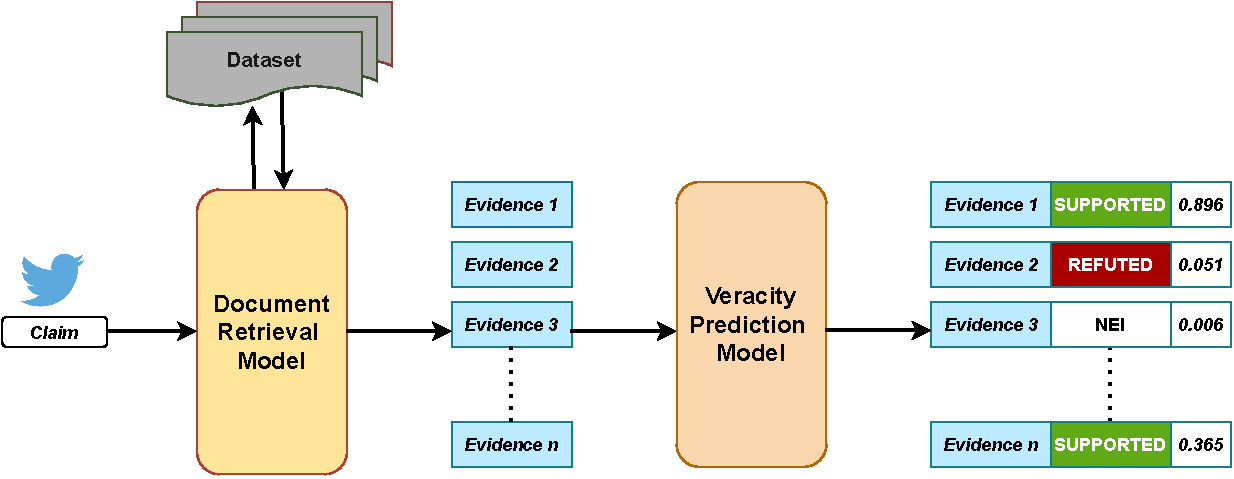
\includegraphics[width=\textwidth]{model.pdf}
    \caption{An overview of the proposed evidence-based claim verification pipeline. The significant components have been highlighted to correspond to the two stages of our experimental setup: (a) a document retrieval module that uses one of the given datasets to retrieve top-k relevant documents for the corresponding input claim, and (b) a veracity prediction module that seeks to establish the retrieved documents' credibility against the input claim.}
    \label{fig:pipeline}
\end{figure*}


\section{Description of the Datasets} 
For our experiments, we adopt two datasets. Their details are shown as follows:
\begin{enumerate}
    \item \textbf{CORD-19 Dataset} \cite{wang2020cord19}: CORD-19 dataset consists of over $\sim500,000$ articles (over $\sim200,000$ containing full text) taken from various scientific publications about COVID-19, SARS-COV2 and other viruses. This dataset provides access to trustworthy scientific sources of information to mitigate the spread of misinformation. %Table \ref{tab:example-cord19} shows some examples from CORD-19 dataset. 

    \item \textbf{LESA Dataset} \cite{gupta2021lesa}: LESA dataset consists of $\sim10,000$ tweets that were mined from various sources and were manually annotated for the binary classification task of claim detection. Furthermore, we develop a validation set -- \textbf{Cla}im \textbf{Ver}ification (\dataset) by selecting a subset of claims from the LESA dataset and annotating those claims with relevant articles that provide additional context for the claim, as shown in Table \ref{tab:example-our-dataset}. These articles are gathered from reliable online news sources and contain additional extensive information that may be used to verify the authenticity of the claim. The articles can ``\textit{Refute}" or ``\textit{Support}" the claim. In other circumstances, the claim may be that the annotated article does not give conclusive evidence. These articles lack sufficient information to support or reject the claim's veracity and hence labelled for ``\textit{Not Enough Information}". These articles are also stored in our global knowledge base of articles along with the articles taken from the CORD-19 dataset.
\end{enumerate}


\section{Our Approach}
Adhering to the standard of automated claim verification and fact-checking systems \cite{thorne-etal-2018-fact}, our proposed approach also consists of a two-step pipeline -- Document Retrieval and Veracity Prediction. In this section, we present the techniques employed for retrieval and veracity prediction components. Besides the current approach, we had also employ alternative techniques using Rapid Automatic Keyword Extraction or RAKE \cite{doi:https://doi.org/10.1002/9780470689646.ch1} and SciSpacy \cite{neumann-etal-2019-scispacy} for keyword extraction and searching our corpus using the extracted keywords. Figure \ref{fig:pipeline} illustrates the general architecture of our proposed claim verification approach. Once a textual claim is submitted, the document retrieval module extracts the top-k relevant documents from the knowledge base. The retrieved documents are then passed to the veracity prediction module that figures out an entailment decision for the claim with respect to the retrieved evidences. 

\begin{table*}[!t]
\centering
\caption{Sample response generated by our proposed system leveraging \dataset\ dataset for extraction.}
\resizebox{\textwidth}{!}
{
\begin{tabular}{c|p{25em}|c|c}
\hline  
    \multicolumn{1}{l}{\bf Claim} \\ 
    
    \multicolumn{4}{l}{\multirow{3}{45em}{Story about how \#HydroxyChloroquine likely help people recover from \#Coronavirus. IMO, it was never touted as the cure but as option for treatment doctors should consider and it appears to work in some cases....39 in one place.}} \\ 
    \multicolumn{4}{c}{} \\
    \multicolumn{4}{c}{} \\ \hline \hline
    % \multicolumn{4}{c}{} \\
    % \multicolumn{4}{c}{} \\ \hline
    \multicolumn{4}{c}{\bf Outputs} \\ \hline
    \bf Technique & \multicolumn{1}{|c|}{\bf Evidence Retrieved\footnotemark} & \bf Label & \bf Veracity \\ \hline
    Ours& \textit{Chloroquine and hydroxychloroquine, a pair of old drugs used to treat and prevent malaria, are the latest compounds to be thrust into the limelight as people tout them as treatments for the novel coronavirus. On Sunday, March 29, the US Department of Health and Human Services accepted 30 million doses of hydroxychloroquine sulfate from Novartis and 1 million doses of chloroquine phosphate from Bayer...The World Health Organization is sponsoring a large international clinical trial called SOLIDARITY to study six drugs that could be rapidly deployed for the fight the coronavirus, including chloroquine and hydroxychloroquine.} & \textcolor{red}{\textsc{Contradiction}} & 0.82737%0882 
    \\ 
    \hdashline
    
    Dense & \textit{As of now, no study says coronavirus can be cured by drinking lots of water or gargling with warm saltwater. Though it is true that warm salt water has long been used as a home remedy to soothe a sore throat, but till now, there is no evidence that it can also ward off the novel coronavirus. A report by fact-check website "Snopes" also says that there is no proof that coronavirus remains in the throat for four days as mentioned in the viral post.} & \textcolor{blue}{\textsc{Neutral}} & 0.99825%43588 
    \\ 
    \hdashline

    Hybrid & \textit{As of now, no study says coronavirus can be cured by drinking lots of water or gargling with warm saltwater. Though it is true that warm salt water has long been used as a home remedy to soothe a sore throat, but till now, there is no esidence that it can also ward off the novel coronavirus. A report by fact-check website "Snopes" also says that there is no proof that coronavirus remains in the throat for four days as mentioned in the viral post.} & \textcolor{blue}{\textsc{Neutral}} & 0.99825%43588  
    \\
    \hline
\end{tabular}}
\label{tab:response}
\end{table*}

\subsection{Document Retrieval}
Inspired by IR systems, the retrieval problem we attempt to address is defined as follows: Given a textual claim $c$ and a set of documents $D$, we aim to retrieve the top-k documents from $D$ relevant to $c$. Our retrieval pipeline consists of two broad categories of retrieval systems, namely Sparse Retrieval and Dense Retrieval.

\begin{enumerate}
\item \textbf{Sparse Retrieval Model:}
Over the years, lexical approaches like TF-IDF and BM25 have dominated textual information retrieval. We also utilize the BM25 scoring function \cite{robertson1995okapi} as the backbone model for sparse retrieval. We use the sparse retrievers for both the \dataset\ as well as CORD-19 datasets. In this case, we also provide an extra option of getting finer-grained results. This step scans through the retrieved article and provides a relevant part of the article. We use a BioBERT \cite{10.1093/bioinformatics/btz682} language model which is pre-trained on large-scale bio-medical corpora. We compute the hidden representation of each paragraph in the article using the language model and calculate its cosine similarity with the hidden representation of the claim. The paragraph with the highest value is then selected.


\item \textbf{Dense and Hybrid Retrieval Models:}
More recently, dense retrieval approaches were proposed to get better retrieval results. They are capable of capturing semantic matches and try to overcome the (potential) lexical gap. Dense retrievers map queries and documents in a shared, dense vector space \cite{gillick2018end}. This allowed the document representation to be pre-computed and indexed. We provide the option of dense retrievers specifically for our \dataset\ dataset. Using dense indexes for CORD-19 dataset is difficult because of the huge size of the corpora. To use the dense and hybrid searchers, we first index our \dataset\ data using the \textsc{Faiss} \cite{JDH17} library. For our dense retriever, we use the simple dense searcher provided by the \textsc{Pyserini} \cite{lin2021pyserini} library while initializing it with COVID-BERT weights. The hybrid searcher uses a combination of sparse and dense retrievers and computes a weighted interpolation of the individual results to arrive at the final rankings. We use the TCT-ColBERT \cite{lin2020distilling} architecture to encode our queries into the same representation space as the encoded documents.
\end{enumerate}

% \begin{table*}[h]
% % \small
%     \caption{NDCG@1, NDCG@10, NDCG@100 on our \dataset\ dataset using various retrieval techniques.}
%     \centering
%     \scalebox{0.90}{
%     \begin{tabular}{l c c c}
%     \hline
%         \bf Technique & \bf NDCG@1 & \bf NDCG@10 & \bf NDCG@100 \\
%         \hline
%         Ours & \bf 24.71 & \bf 36.75 & \bf 45.73 \\\hline
%         CrossEncoder MS Marco & 22.99 & 35.41 & 35.41 \\
%         CrossEncoder CovidBERT & 3.41 & 15.04 & 15.04 \\
%         SentenceBERT MS Marco & 18.97 & 32.09 & 32.58 \\
%     \hline
%     \end{tabular}}
%     \label{tab:ndcg_scores}
% \end{table*}

\begin{table*}[h]
% \small
    \caption{%NDCG@1, NDCG@10, NDCG@100, MAP@1, MAP@10, MAR@1 and MAR@10 
    Performance of various retrieval techniques on \dataset\ dataset. (NDCG: Normalized Discounted Cumulative Gain, MAP: Mean Average Precision and MAR: Mean Average Recall)}
    \centering
    \scalebox{0.80}{
    \begin{tabular}{l c c c c c c c c}
    \hline
        \bf Technique & \bf NDCG@1 & \bf NDCG@10 & \bf NDCG@100 & \bf MAP@1 & \bf MAP@10 %& \bf MAP@100 
        & \bf MAR@1 & \bf MAR@10\\
        \hline
        Ours & \bf 24.71 & \bf 36.75 & \bf 45.73 & \bf 24.71 & \bf 32.14 %& 33.76 
        & \bf 24.71 & \bf 51.72\\\hline
        CrossEncoder MS Marco & 22.99 & 35.41 & 35.41 & 22.99 & 31.12 % & 31.12 
        & 22.99 & 48.85\\
        CrossEncoder CovidBERT & 3.41 & 15.04 & 15.04 & 3.41 & 3.41 % & 8.95 
        & 3.49 & 36.36 \\
        SentenceBERT MS Marco & 18.97 & 32.09 & 32.58 & 18.97 & 26.83 % & 26.98 
        & 18.97 & 49.43 \\
    \hline
    \end{tabular}}
    \label{tab:ndcg_scores}
\end{table*}


\begin{figure*}[h]
    \centering
    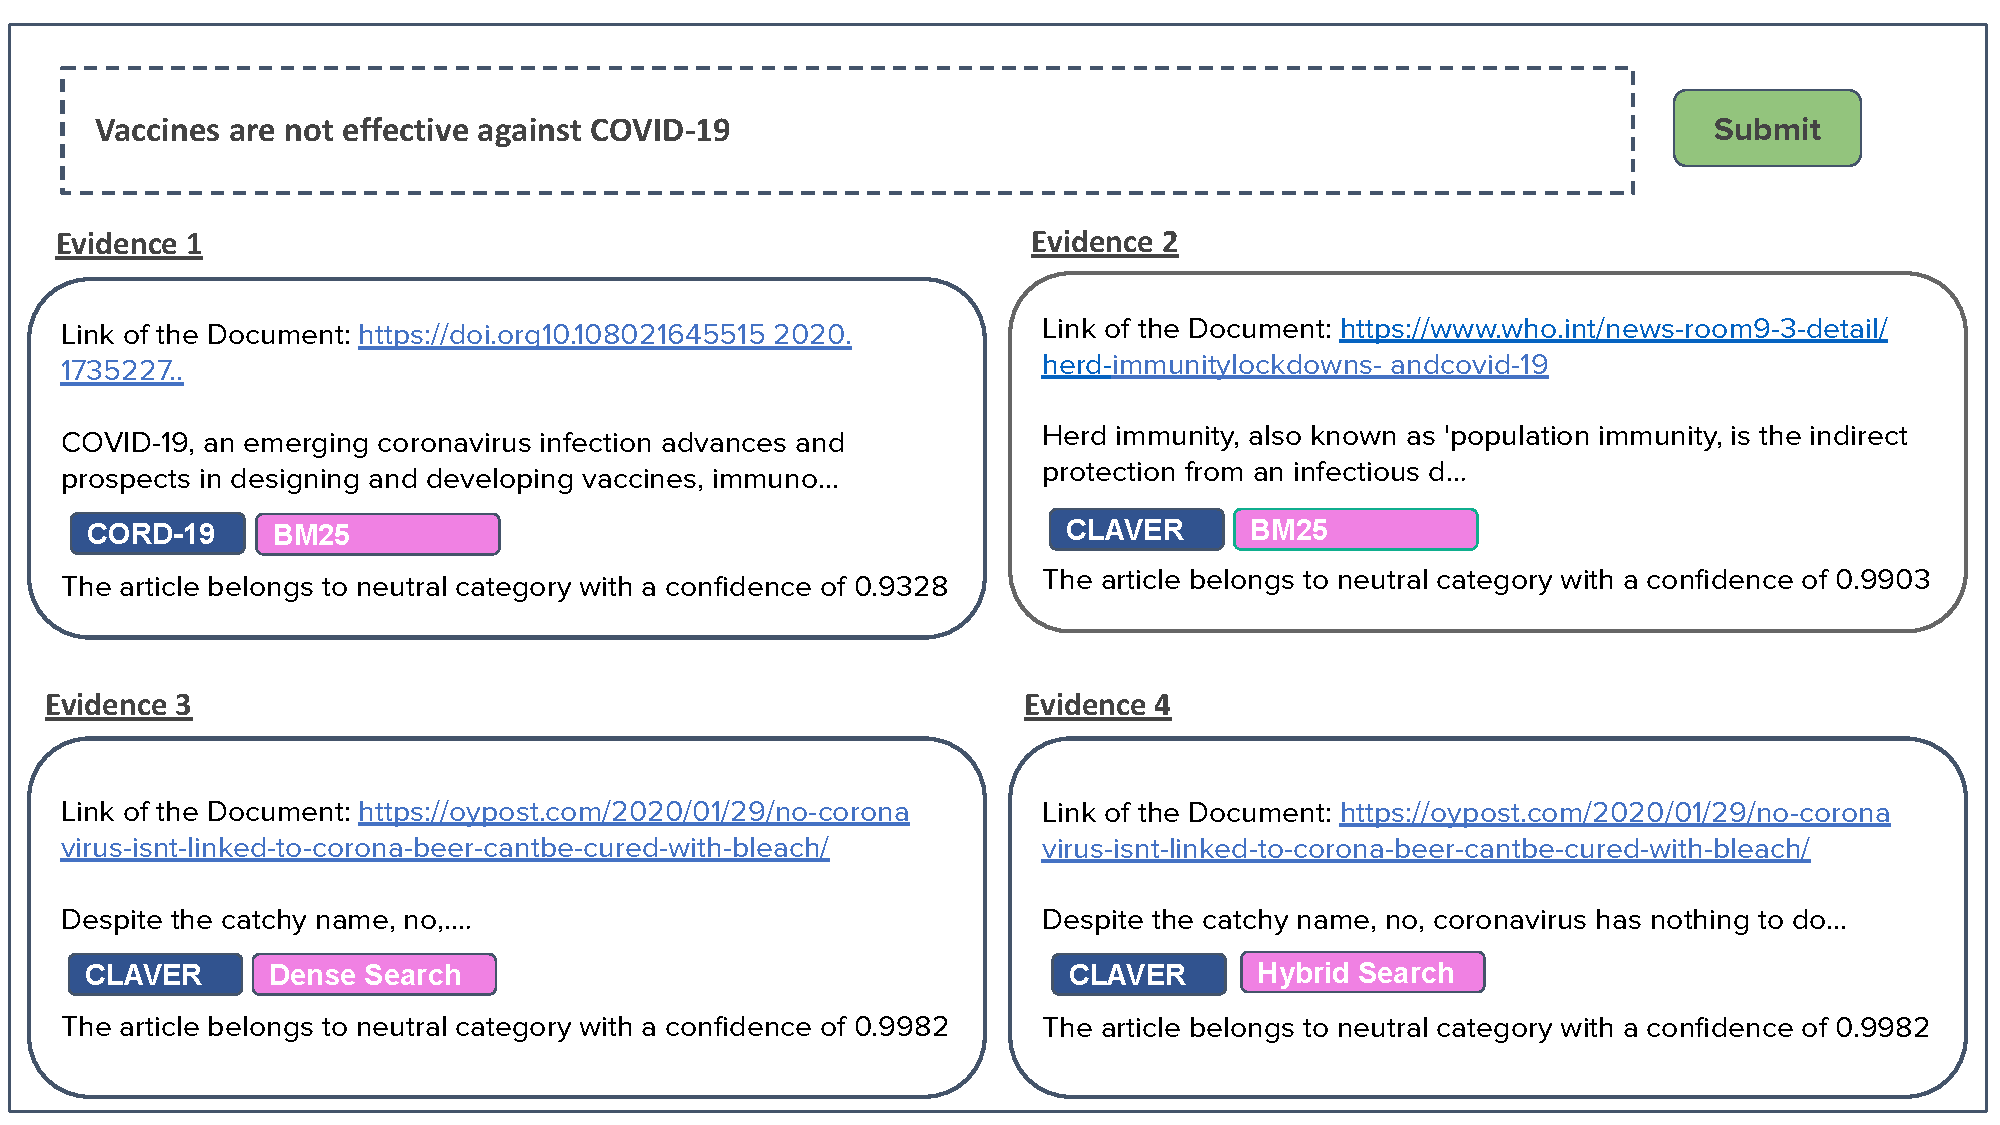
\includegraphics[width=\textwidth]{tool-output.pdf}
    \caption{User-interface of our proposed tool after the claim has been submitted.}
    \label{fig:sample}
\end{figure*}


% % \vspace{-2em}
% \begin{table*}[h]
% % \small
%     \caption{Mean average precision (MAP) and mean average recall (MAP) for various techniques.}
%     \centering
%     \scalebox{0.85}{
%     \begin{tabular}{l c c c c }
%     \hline
%         \bf Technique & \bf MAP@1 & \bf MAP@10 %& \bf MAP@100 
%         & \bf MAR@1 & \bf MAR@10 \\
%         \hline
%         Ours & \bf 24.71 & \bf 32.14 %& 33.76 
%         & \bf 24.71 & \bf 51.72 \\\hline
%         CrossEncoder MS Marco & 22.99 & 31.12 % & 31.12 
%         & 22.99 & 48.85 \\
%         CrossEncoder CovidBERT & 3.41 & 3.41 % & 8.95 
%         & 3.49 & 36.36 \\
%         SentenceBERT MS Marco & 18.97 & 26.83 % & 26.98 
%         & 18.97 & 49.43 \\
%     \hline
%     \end{tabular}}
%     \label{tab:map_recall_scores}
%     % \vspace{-1em}
% \end{table*}
% % \vspace{-2em}




\subsection{Veracity Prediction}
Given a claim and the evidence gathered through document retrieval system, veracity prediction module seeks to establish the evidence's credibility in terms of a veracity score. To verify the veracity of our retrieved articles, we leverage a BART-based \cite{lewis-etal-2020-bart} Natural Language Inference (NLI) model that returns one of the three classes for each claim-evidence pair: Entailment, Neutral and Contradiction (as shown in Table \ref{tab:response}). The mapping of these labels with our use case is done in the following way:
\begin{itemize}
    \item If the model outputs `Entailment', it means that the given claim's veracity can be positively supported by the retrieved article.
    \item If the model outputs `Contradiction', it means that the given claim's veracity is refuted by the retrieved article which makes the claim dubious.
    \item If the model outputs `Neutral', it means the retrieved article does not provide enough evidence to either support or refute the claim.
\end{itemize}


\section{Evaluation}


We compare the findings of our retrieval system BM25 to those of other existing systems. We employ a collection of claims and ground-truth labels from our \dataset\ dataset for quantitative evaluation. The test data set consists of claims excluded from the knowledge base in the retrieval phase. For this, we develop a manually annotated dataset with $\sim1000$ claims obtained from Twitter and build a knowledge-base of $\sim400$ articles from reliable sources, equipping a testing ground to validate the results. Table \ref{tab:ndcg_scores} presents experimental results based on Normalized Discounted Cumulative Gain (NDCG@k) scores, Mean Average Precision (MAP@k) and Mean Average Recall (MAR@k) scores for different values of k. We find that using BM25 outperforms all other baseline systems for retrieval task. The NDCG@100 score of the BM25 retrieval model improves the baseline method by more than 10\% out of the whole testing set.  We find that BM25 detects relevant snippets with higher precision and recall than other existing retrieval systems.  %Mean Average Precision on the first 5 retrieved claims (MAP@5) is used to assess the quality of the rankings.

\footnotetext{Links of article sources can be found at: \url{https://cutt.ly/lFwsxXa}}



\section{Demonstration}
In this section, we demonstrate how our proposed claim verification pipeline works. Figure \ref{fig:sample} depicts an example claim as well as the model's output results. Users enter a claim into our system as a query, and the system evaluates whether or not it is a validated claim. In practice, the system takes somewhere around 20 and 80 seconds to execute a single user query, depending on the number and length of articles obtained by the search engine.

The input section of our tool, as shown in Figure \ref{fig:sample}, provides a query text box where the user can enter any natural language text as an input claim for evaluation, as well as a specific configuration to limit the number of articles to be retrieved. Following the submission of the claim, the tool's back-end server does its analysis. It returns three sets of outputs: (i) a set of articles employing the various approaches, (ii) a claim category, and (iii) a veracity score. The output also presents the technique utilized for retrieval (pink) and from which knowledge base the shreds of evidence were extracted (blue). The most intriguing aspect of the system is that it links resources from the web, where the article was retrieved, allowing individuals to make their own decisions based on them. 
 
Not all information is equally reliable, and sometimes even the trusted sources contradict one another. This calls into question the assumptions behind most current fact-checking research, which relies on a single authoritative source. As a result, we offer results for a common claim from several models and knowledge bases. For demonstration, we practice the widely spread claim \textit{``Vaccines are not effective against COVID-19"} as an input as shown in Figure \ref{fig:sample}, and the tool returned the top-ranked shreds of evidence. The first two pieces of evidence come from the BM25 model, which was run on the CORD-19 dataset and our data, respectively. Furthermore, evidences 3 and 4 collected articles from our dataset using a dense and hybrid retrieval strategy, respectively. We can see that all four pieces of evidence assigned the same label to the claim, but their truthfulness scores differed from each other. 





\section{Conclusion}
In this work, we verged upon claim verification on online social media towards coping with misinformation. We bestowed a claim verification system that evaluates the authenticity of a user-supplied query claim and justifies the verdict corroborating evidence. We explored multiple retrieval methodologies and published user research findings, demonstrating the utility of the BM25 method. Unlike other tools, our system learns the distributed representations to encapsulate the semantic relations between the claim and the evidence. Our approach uses a two-step training process to provide a high-quality veracity score as well as best-suited articles, leveraging data from formal articles and web-based informal texts. We have made the source codes and the dataset public at the following link: \url{https://github.com/LCS2-IIITD/claim_verification}.

\section*{Acknowledgements}
T. Chakraborty would like to acknowledge the support of the Ramanujan Fellowship, and ihub-Anubhuti-iiitd Foundation set up under the NM-ICPS scheme of the Department of Science and Technology, India. M. S. Akhtar and T. Chakraborty thank Infosys Centre for AI at IIIT-Delhi for the valuable support.

% Entries for the entire Anthology, followed by custom entries
\bibliography{anthology,custom}
\bibliographystyle{acl_natbib}

\end{document}
